% vim: set spelllang=fr:
\setchapterpreamble[ur][.7\textwidth]{%
  \dictum[Robin Hobb, \textit{La Voie magique}]{%
      Je levai les yeux vers leurs visages effrayés et me rendit compte qu'ils parlaient -- non, ils hurlaient presque ; [...] quelqu'un demandait sans cesse : « Que s'est-il passé ? Que s'est-il passé ? » Je fus soudain frappé du manque de grâce de la parole : tous ces mots rattachés les uns aux autres, que chaque bouche prononçait différemment... Et c'était ainsi que nous communiquions ?}}
\chapter{\verbenet{} : une traduction de VerbNet}
\label{ch:verbnet}

La ressource anglaise VerbNet (section~\ref{presentation_verbnet}) correspond à
nos objectifs (section~\ref{objectifs_these}) mais n'existe qu'en anglais :
c'est pourquoi nous présentons dans ce chapitre sa traduction vers le français,
\verbenet{}\footnote{Le nom vient de la prononciation à la française qui
"rajoute" un \emph{e}. Le $\ni$ est là pour bien marquer ce \emph{e} et ainsi
essayer d'éviter la confusion avec VerbNet.}. Une partie conséquente de cette
article provient d'articles déjà publiés
\citep{danlos2014vers,pradet2014adapting}.

La construction de cette ressource s'est faite en trois étapes. Nous avons
d'abord traduit vers le français les membres des classes de premier niveau dans
VerbNet en utilisant des ressources linguistiques qui encodent des informations
syntaxiques et sémantiques sur les verbes du français (section~\ref{first}). La
deuxième étape, toujours en cours, est l'adaptation des frames VerbNet vers le
français et la réorganisation les classes de VerbNet en fonction de ces frames,
ce qui pose divers problèmes que nous décrirons en partie ici
(section~\ref{second}). La troisième étape sera l'occasion de valider les
membres français de chaque classe (section~\ref{third}).

Notre traduction de VerbNet est liée aux deux ressources linguistiques que nous
utilisons, Les Verbes Français et le Lexique-Grammaire. La ressources est aussi
ouverte : nous voulons encourager les contributions externes avec notre outil
basé sur le web. Nous souhaitons aussi faciliter l'utilisation de la ressource
en utilisant le même format XML que le VerbNet anglais.

\section{Construction de \verbenet{}}

Notre principe de base est que la hiérarchie supérieure de VerbNet doit être
aussi proche que possible de celle de VerbNet et ses 270 classes. Néanmoins,
certaines classes peuvent disparaître. Ceci peut être dû à des raisons purement
morphologiques. Une classe VerbNet ne contenant que des verbes dénominaux n'a
pas d'équivalent en français. C'est le cas de \texttt{pit-10.7} avec des verbes
tels que \emph{bark} et \emph{bone} ou \texttt{week-end-56} et ses verbes
\emph{week-end} ou \emph{december}. Par contre, \texttt{debone-10.8} et ses
verbes formés par le préfixe \emph{dé-} plus un nominal (\emph{debark, debone})
a un équivalent français avec les préfixes \emph{dé-} ou \emph{é}
(\emph{déveiner}, \emph{équeuter}).

Étant donné ce principe de base, la construction de \verbenet{} se fait en
trois étapes.

\subsection{Première étape}\label{first}

La première étape pour construire \verbenet{} est de déterminer quels verbes
français appartiennent à une des 270 classes de VerbNet. Ceci a été fait en
trois étapes.

\begin{enumerate}

    \item Pour une classe VerbNet donnée \Ce{}, nous assignons manuellement les
        classes LVF \Clvf{} et les classes LG \Clg{} qui correspondent à sa
        définition sémantique : nous assignons par exemple {\color{red}L3b} et
        {\color{green}38LD} à {\color{blue}put-9.1} et assignons
        {\color{red}M1a} et {\color{green}32CL ou 32R3 ou 32C} à
        {\color{blue}body\_internal\_motion-49}.

    \item Nous utilisons deux dictionnaires bilingues (SCI-FRAND-EURADIC et le
        Wiktionnaire) qui fournissent la liste \Ltrad{} des traductions
        françaises des verbes anglais appartenant à \Ce{} et ses sous-classes.

    \item Les verbes français de la classe \Ce{} sont alors simplement les
        verbes appartenant à la fois à \Ltrad{}, \Clvf{} et
        \Clg{}\footnote{Quand cette intersection est vide, c'est la liste
        non-vide (soit \Clvf{} soit \Clg{}) qui est choisie}. Par exemple,
        \emph{mettre}, \emph{poser} et \emph{installer} sont des verbes
        français de {\color{blue}put-9.1}).

\end{enumerate}

Cette étape a été exécutée rapidement et a donné des résultats encourageants :
en ne gardant que les verbes à l'intersection de \Ltrad{}, \Clvf{} et \Clg{},
les résulstats sont précis et cohérents d'un point de vue sémantique et
syntaxique. Par exemple, la classe {\color{blue}scribble-25.2} contient 18
verbes en anglais : elle est associée à la classe LVF {\color{red}R3a.1} et à
la table LG {\color{green}32A}, ce qui conduit à une liste de 16 verbes
français : \emph{composer}, \emph{couper}, \emph{donner}, \emph{exécuter},
\emph{fabriquer}, \emph{faire}, \emph{forger}, \emph{former}, \emph{imprimer},
\emph{lever}, \emph{produire}, \emph{reproduire}, \emph{sculpter},
\emph{tailler}, \emph{tirer} et \emph{tracer}. Tous ces verbes sont valides
pour cette classe.  Cette méthode produit un lexique de 4058 verbes (2128
verbes distincts).

% TODO Évaluer automatiquement à l'aide de la validation des verbes

\subsection{Deuxième étape}\label{second}

% TODO stats sur un VerbNet importé, pas sur VerbeNet à moitié fini
La deuxième étape de la construction de \verbenet{} s'est avérée beaucoup plus
fastidieuse que la première. Pour chacune des 500 classes et sous-classes, nous
déterminons quand cela est possible :

\begin{itemize}

    \item les frames valides pour le français avec des ajustements possibles
        pour les rôles thématiques et les restrictions de sélection,

    \item les sous-classes en français en réorganisant si besoin la hiérarchie
        de l'anglais dans le but d'assigner les verbes obtenus à l'étape 1 à
        une des sous-classes.

\end{itemize}

Cette étape a demandé le développement d'un outil d'édition
(section~\ref{toolquentin}) pour assister le travail lexicographique. Ensuite,
il a fallu définir des principes de base sur les frames françaises quand elle
diffèrent des frames anglaises (section~\ref{princp}). Finalement, une étude
fine au cas par cas révèle des différences difficiles à traiter entre l'anglais
et le français (section~\ref{subsubsec:casebycase}).

\subsubsection{Outil d'édition de \verbenet{}}\label{toolquentin}

Nous avons du développer un outil permettant d'éditer collaborativement
VerbNet\footnote{Cet outil est libre et disponible sur GitHub :
\url{https://github.com/aymara/verbenet-editor}.}. Cet outil est en fait un
site web présentant VerbNet : ses classes, ses frames, ses verbes, etc.  Tous
les éléments sont modifiables, ce qui permet aux lexicographes de se concentrer
sur les problèmes lexicographiques sans avoir à se préoccuper de la
représentation des données. Le site web est réalisé avec Django, un framework
web Python. VerbNet est stocké dans une base de donnée PostgreSQL. Avant de
commencer l'édition, nous avons commencé par charger VerbNet et les mappings
réalisés lors de la première étape. L'édition elle-même se fait classe de Levin
par classe de Levin. Par exemple, nous avons traité ensemble les classes
{\color{blue}throw-17.1} et {\color{blue}pelt-17.2} parce qu'elles font toutes
les deux partie de la «~super-classe~» 17 : Throwing. Plusieurs classes faisant
partie d'une même super-classe sont souvent liées et il faut les comprendre
dans leur ensemble avant de commencer l'édition. Pour chaque classe, nous
pouvons éditer ses frames, ajouter ou supprimer des sous-classes ou des frames.
Par exemple, pour la suppression, toutes les frames impliquant un conatif, un
datif ou une alternance bénéfactive peuvent être systématiquement supprimées :
ces alternances n'existent pas en français.

\begin{figure}

    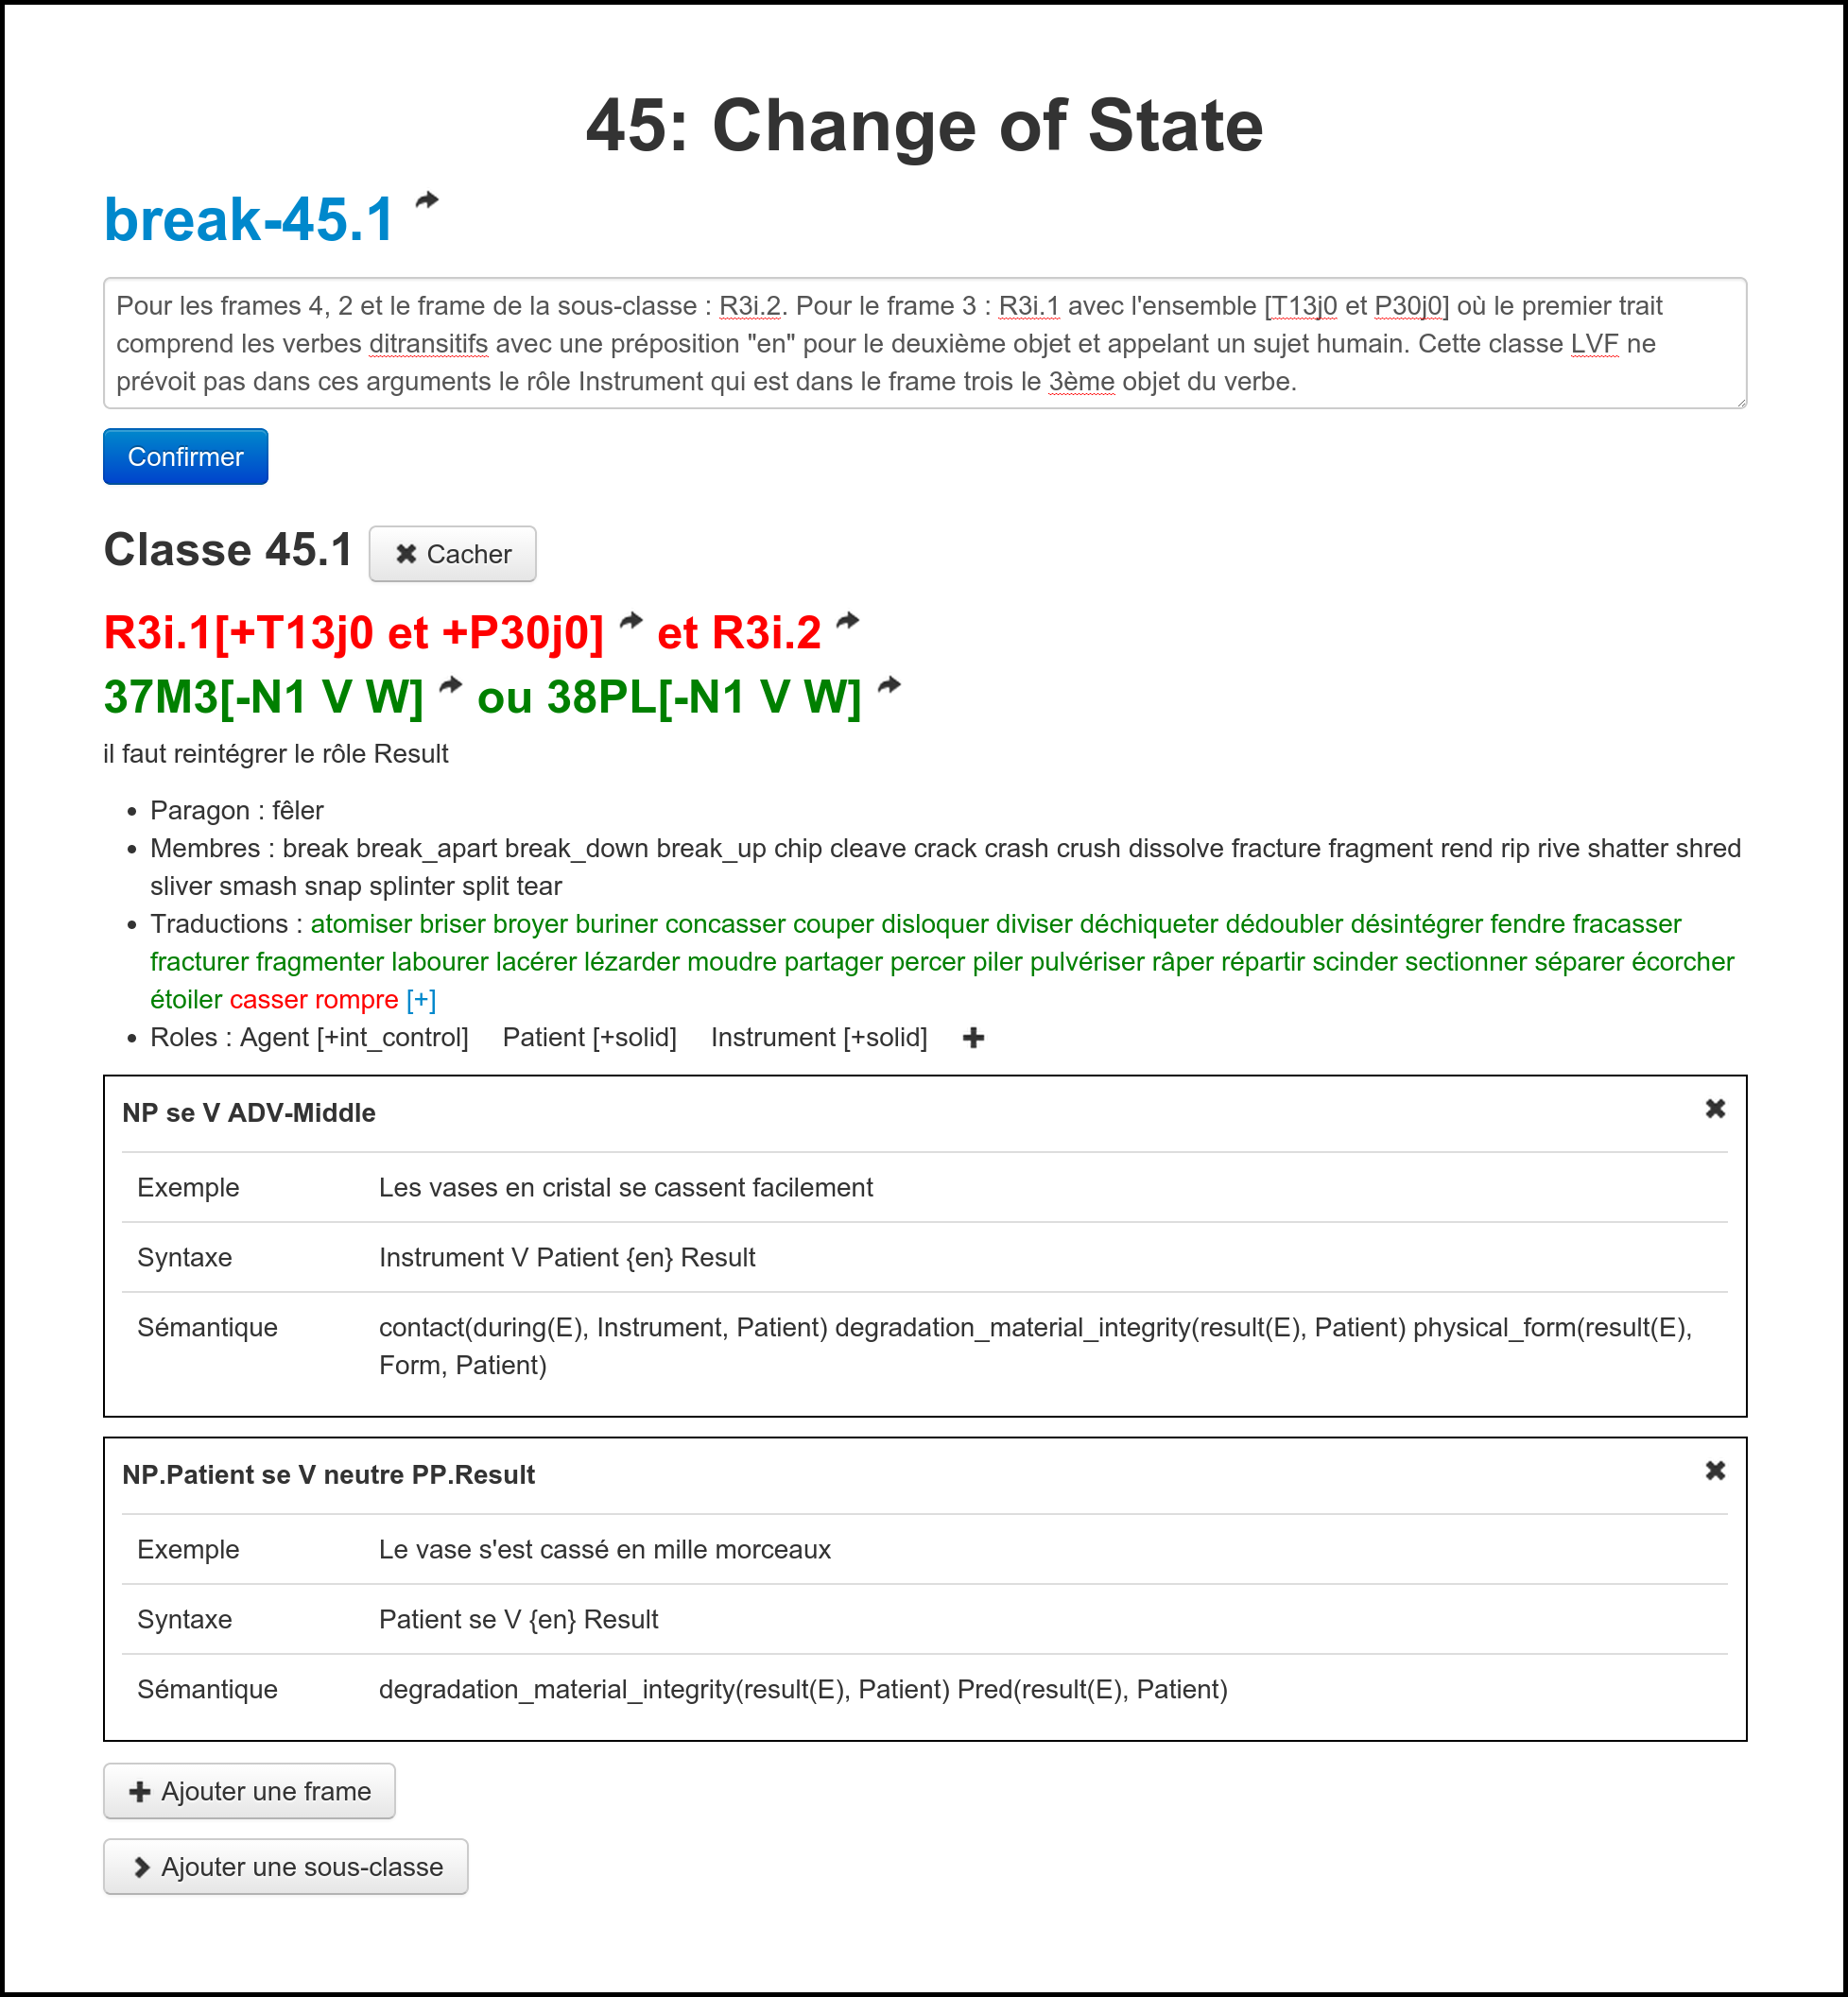
\includegraphics[width=\textwidth]{fig/tool_screenshot_2014-09-12.png}

    \caption{\label{tool}Interface web pour analyser et modifier \verbenet{}.
        Chaque frame peut être modifiée et les classes peuvent être
        réorganisées. Les traductions en violet apaprtiennent à l'intersection
        de \Clvf{}, \Clg{} et \Ltrad{} (section~\ref{first}), les traductions
        en rouge (respectivement en vert) uniquement à \Clvf{} et \Ltrad
        (respectivement uniquement à \Clg{} et \Ltrad{}). La description de
        {\color{blue}break-45.1} est en cours de modification : en cliquant sur
        'Confirmer', la modification sera prise en compte rapidement sans avoir
    à recharger la page pour éviter d'interrompre le travail lexicographique.}

\end{figure}

Avec l'aide de cet outil (illustré à la Figure~\ref{tool}), la deuxième étape
peut s'avérer très simple. Par exemple, les quatre sous-classes de
{\color{blue}image-creation-25} ont des classes directement équivalentes en
français, donc les seules choses à faire sont de traduire les exemples en
français avec les bonnes prépositions. Par exemple, dans la classe
{\color{blue}illustrate-25.3}, il a fallu remplacer \emph{with} par la
combinaison de \emph{de} et \emph{avec}.

\subsubsection{Principes sur les frames}\label{princp}

Nous avons jusqu'ici identifié deux différences principales entre le codage des
frames anglaises et françaises.

La première différence concerne les sous-structures, c'est-à-dire les frames
avec un complément manquant tel que \emph{NP V} (Luc gravait) dans
{\color{blue}image-impression-25.1}. C'est en effet ici une sous-structure de
\emph{NP V NP.Destination} (Luc gravait les anneaux). Le codage de telles
sous-structures est difficile à justifier quand il est basé sur l'introspection
linguistique et nécessite une étude de corpus. Nous ne savons pas comment ce
codage a été fait dans VerbNet et n'avons pas à notre disposition de corpus
français permettant de répondre à la question. Nous avons donc décidé pour le
moment de supprimer toutes les sous-structures de \verbenet{}. Par exemple,
dans la classe {\color{blue}remove-10.1}, VerbNet encode non seulement NP V NP
PP.Source PP.Destination (\emph{Doug removed the smudges from the tabletop})
mais aussi NP V NP (\emph{Doug removed the smudges}). \verbenet{} n'inclut que
la première frame, il est implicite que la seconde existe : une application
doit donc l'inférer automatiquement à partir de la première sans intervention
manuelle\footnote{Cependant, ce principe ne s'applique pas aux verbes acceptant
un seul complément locatif double «~from here to there (un seul
complément PP.Source PP.Destination)~» sans accepter un seul complément source
(PP.Source), tout en acceptant un seul complément destination
(PP.Destination) : \emph{Fred a transferré le vin de la cruche en pierre vers
la cruche en terre cuite, *Fred a transferré le vin de la cruche en pierre,
Fred a transferré le vin vers la cruche en terre cuite}. Dans ce cas
exceptionnel, les sous-structures sont codées explicitement.}.

La deuxième différence concerne l'ordre des compléments. VerbNet encode parfois
des frames qui ne diffèrent que par l'ordre des compléments, par exemple dans
{\color{blue}bring-11.3} les frames NP V NP PP.Destination NP (\emph{Nora
brought to lunch the book}) et NP V NP PP.Destination (\emph{Nora brought the
book to the meeting}). En français, l'ordre des compléments dépend d'un certain
nombre de facteurs syntaxiques et sémantiques \citep{thuilier2012contraintes},
mais ne dépend pas a priori d'un facteur lexical : il ne dépend pas du verbe
qui gouverne les compléments. C'est pour cette raison que \verbenet{} n'encode
qu'un frame dans ces cas, ici seulement \emph{NP V NP PP.Destination}
(\emph{Nora a apporté le livre au meeting}) avec l'objet direct avant le
syntagme prépositionnel. C'est à l'utilisateur de la ressource de considérer
que l'autre option (\emph{NP V PP.Destination NP}, \emph{Nora a apporté au meeting
le livre}) est tout aussi valable.

\subsubsection{Travail au cas par cas}\label{subsubsec:casebycase}

Dans certains cas, cette deuxième étape pose des difficultés, et ce pour deux
raisons principales. Premièrement, certaines différences sémantiques entre
verbes communes à l'anglais et au français sont prises en comptes par VerbNet
mais ni par LVF ni par le LG. Par exemple, dans les verbes de \emph{Sendying
and Carrying} (la super-classe 11), les verbes dans les classes
{\color{blue}bring-11.3}, {\color{blue}carry-11.4} et {\color{blue}drive-11.5}
décrivent un mouvement accompagné (non seulement le Theme mais aussi l'Agent
changent de location comme dans \emph{Pamela drove packages to NY}). Au
contraire, les autres classes ({\color{blue}send-11.1} et
{\color{blue}slide-11.2}) décrivent un mouvement non accompagné (seul le Thème
se déplace comme dans \emph{Pamela sent packages to NY}). Dans les ressources
françaises, des classes existent pour des verbes avec un changement de location
pour un Thème causé par un Agent, mais rien n'est codé pour le mouvement de
l'Agent. Face à cette difficulté, deux solutions se présentent.

\begin{itemize}
    \item soit réaliser une étude complète des verbes français de \emph{Sending
        and Carrying} pour distinguer les mouvements accompagnés et
        non-accompagnés,
    \item soit ignorer purement et simplement cette différence sémantique.
\end{itemize}

Dans ce cas, nous avons opté pour la seconde solution étant donné que cette
information n'est pas directement utile pour l'annotation en rôles
sémantiques\footnote{Il semble par ailleurs que pour certains verbes anglais,
    l'Agent peut être ou non en mouvement : voir la différence entre les
classes VerbNet {\color{blue}carry-11.4} et {\color{blue}carry-11.4-1}.}.
C'est un choix discutable : si pour notre application la position de l'Agent
avait eu un intérêt, comme ce pourrait être le cas en implication textuelle,
une étude plus complète aurait été souhaitable. Nous préférons nous concentrer
sur la sortie d'une première version de VerbNet, quitte à revenir sur certains
choix par la suite.

Le fait d'ignorer cette différence nous mène à adopter dans \verbenet{} une
hiérarchie différente de VerbNet pour la super-classe 11 : il n'y a pas
d'équivalent dans \verbenet{} de la classe {\color{blue}carry-11.4}, les verbes
de cette classe devant être placés dans les classes {\color{blue}send-11.1} et
{\color{blue}slide-11.2}. Par ailleurs, il n'y a pas d'équivalent en français
de la classe {\color{blue}bring-11.3} qui contient uniquement les deux verbes
\emph{bring} et \emph{take} avec une direction spécifiée déictiquement
\citep[page 135]{levin1993english} parce que les déictifs locatifs français
\emph{ici} et \emph{là} n'ont pas le fonctionnement de \emph{here} et
\emph{there} en anglais\footnote{En français, \emph{Je suis là} peut signifier
\emph{Je suis ici}.}.

La seconde source principale de difficultés provient de différences cruciales
entre le français et l'anglais. Il existe des problèmes de traductions entre
ces deux langues qui sont bien connus et documentés, comme la traduction des
verbes de mouvement (par exemple \emph{John swam across the river}
$\rightarrow$ \emph{Jean a traversé la rivière à la nage}). Sans traiter ces
cas connus, nous discutons ici de situations plus subtiles, comme par exemple
avec les verbes de changement de possession. Dans VerbNet, dix classes sont
dédiées à ces verbes. Une telle hiérarchie est impossible en français. Sans
tout détailler, insistons sur ces quelques points :

\begin{itemize}

    \item L'absence d'alternances datif et bénéfactif en français implique que
        les classes VerbNet {\color{blue}give-13.1} et
        {\color{blue}contribute-13.2} doivent probablement être fusionnées en
        français.

    \item La différence sémantique entre {\color{blue}give-13.1} et
        {\color{blue}future\_having-13.3} (HAS-POSSESSION vs. FUTURE-POSESSION)
        est peut-être trop subtile et pourrait être ignorée.

    \item La préposition \emph{with} dans la frame correspondant à \emph{Agent
        V Recipient \{with\} Theme} utilisée en {\color{blue}fulfilling-13.4-1}
        et {\color{blue}fulfilling-13.4-2} doit être remplacée par \emph{en}
        et/ou \emph{de} suivant le verbe (e.g. \emph{Luc livre Max en/*de
        lait}, \emph{Luc équipe Max en/de téléviseurs}, \emph{Luc dote Max
        *en/de téléviseurs}), ce qui nécessite une réorganisation en
        sous-classes pour distinguer ces verbes.

\end{itemize}

En conclusion, il s'avère que rentrer dans le détail des frames lors de cette
deuxième étape nous a mené a faire évoluer la hiérarchie de \verbenet{}.
Cependant, nous essayons de limiter les modifications quand il est impossible
de faire autrement afin de profiter au maximum de VerbNet et pour pouvoir
profiter du lien entre les deux ressources.

\subsection{Troisième étape}
\label{third}

La troisième étape  est de valider manuellement pour chaque classes les verbes
proposés par correspondance de ressources en supprimant les verbes erronés et
en rajoutant les verbes manquants afin que la ressource ait été entièrement
validée manuellement. Aucun verbe n'est ajouté manuellement : les annotateurs
cliquent directement sur les verbes inférés pour les valider ou les invalider.
Les traductions des dictionnaires étant très productives, les verbes souhaités
sont systématiquement dans les traductions proposées, même s'ils peuvent être
absent des correspondances LADL, LVF ou les deux. Dans les rares cas où un
verbe souhaité n'est pas trouvé, c'est une occasion de contribuer au
Wiktionnaire pour le rajouter.

\section{Conclusion}

Nous avons présenté une méthode pour adapter la ressource syntaxico-sémantique
VerbNet vers une nouvelle langue. Cette méthode combine l'automatisation du
transfert de frames, la traduction automatique du lexique et une expertise
linguistique. Nous avons appliqué cette méthode au français et avons atteint un
point où cette ressource est validée et le travail systématique sur chaque
classe est en cours. Nous reconnaissons les différences qui existent entre les
langues : la structure de \verbenet{} n'est pas exactement celle de VerbNet.

% TODO exporter dans un format libre et mettre quelque part !
